\chapter{Results}

\section{Dataset}
The dataset is made up of 16 pages from a Tamil
encyclopedia. However, we considered only two pages
out of it for the whole experiment and also we segregated intractable characters from the rest.
One page is used for creating the model and other page is used for testing.

\section{Tools}
\subsection{Tesseract OCR Architecture}

\begin{figure}\centering
\includegraphics[scale=0.4]{./img/arch}
  \caption{Architecture of tesseract engine, courtesy of Ray Smith}\label{TESS}
\end{figure}

Tesseract has basically uses two import modules for character recognition.
\begin{itemize}
	\item Character Chopper.
	\item Character Associator.
\end{itemize}
But additionally it makes use of Static classifier, Adaptive classifier and Dictionary for recognition.
\subsection{Module description for making changes}
\begin{itemize}
	\item api -- the plain api's that tesseract avails for creating custom OCR like ocropus gets into this directory.
	\item ccstruct -- the common data structure that tesseract uses gets into this directory.
	\item classify -- this directory contains modules for character classification.
	\item cutil -- this directory contains file handling and heap management routines.
	\item dict -- this directory contains word sense disambiguation routines for error correction and proper classification.
	\item tessdata -- this is ideally the place where training data resides before it gets into /usr/share/tessdata or /usr/local/share/tessdata 
	depending upon your installation configuration option.
	\item textord -- this directory contains modules for preprocessing.
	\item wordres -- this directory contains modules for recognition of characters.
	\item cmain -- this directory contains essential modules for a fully functional OCR.
	\item java -- this directory contains the piccolo client stub for interactive mode. It makes uses of the piccolo package for displaying word segmentation and for editing box files. It is available at \url{http://www.cs.umd.edu/hcil/jazz/team/index.shtml}.Make sure that piccolox.jar is in the classpath.
\end{itemize}
\begin{description}
\item[Classpath:] bash$>$ export CLASSPATH=\$CLASSPATH:/path/to/my/piccolo.jar
\end{description}

\subsection{Classification}
It does Polygonal approximation of each image to get rid of noise and extracts feature from it for classification. It uses static classifier for classifying broken characters and it can be time consuming.
\subsection{Features}
It can handle unicode and it already supports bunch of languages.
\subsection{Running Tesseract}
We can run Tesseract either in Normal or Interactive mode. In the interactive mode, the user could visualize the chopped blobs and if needed could edit the bounding box of each of the characters in the document image.
\begin{description}
	\item[Normal mode:] bash$>$ tesseract sam.tif out [-l eng ]
	\item[Interactive mode:] bash$>$ tesseract sam.tif out [-l eng ] inter
\end{description}
\begin{figure}\centering
\includegraphics[scale=0.5]{./img/segment}\\
  \caption{Tesseract engine in interactive mode}\label{TESSS}
\end{figure}

In the above commands 'eng' stands for English. It is the language code. By default tesseract uses English as the recognition language. However, it doesn't matter in our case because we basically use it
only for extracting the bounding box.
The output is written to out.txt in this case.
\subsection{Extracting bounding box information}
If you want Tesseract to do only preprocessing and get the blob information, you could easily do that as follows.
\begin{itemize}
	\item bash$>$ tesseract sam.tif out makebox
\end{itemize}
The blob information is written into out.box. After this you could use our blob extractor to get the blobs to be used for recognition.
\begin{table}[!t]\center
\begin{tabular}{cccccc}
\toprule
\textbf{Junk} & \textbf{Top} & \textbf{Left} & \textbf{Right} & \textbf{Bottom} & \textbf{Page no} \\
\midrule
@ &865 & 2893  & 883 & 2913  &0 \\
Q &867 &2875 &878 &2885  &0 \\
w &879 &2875 &889 &2885 &0 \\
w &867 &2852 &881 &2862 &0 \\

\bottomrule
\end{tabular}
  \caption{Sample bounding box information for four blobs in a page}\label{BBOX}
\end{table}
\subsection{Using Moshpytt with Tesseract}
As mentioned earlier, Moshpytt could greatly reduce our work of creating training samples for new languages with tesseract. The tool can also be used to edit the bounding box related information. It is written in python and we use it only to edit bounding box information since we are using our oown method based on RPT and SVMTC for character recognition. It can be invoked by running 
\begin{description}
	\item[ bash$>$] python moshpytt.py \#editing box file
\end{description}
	
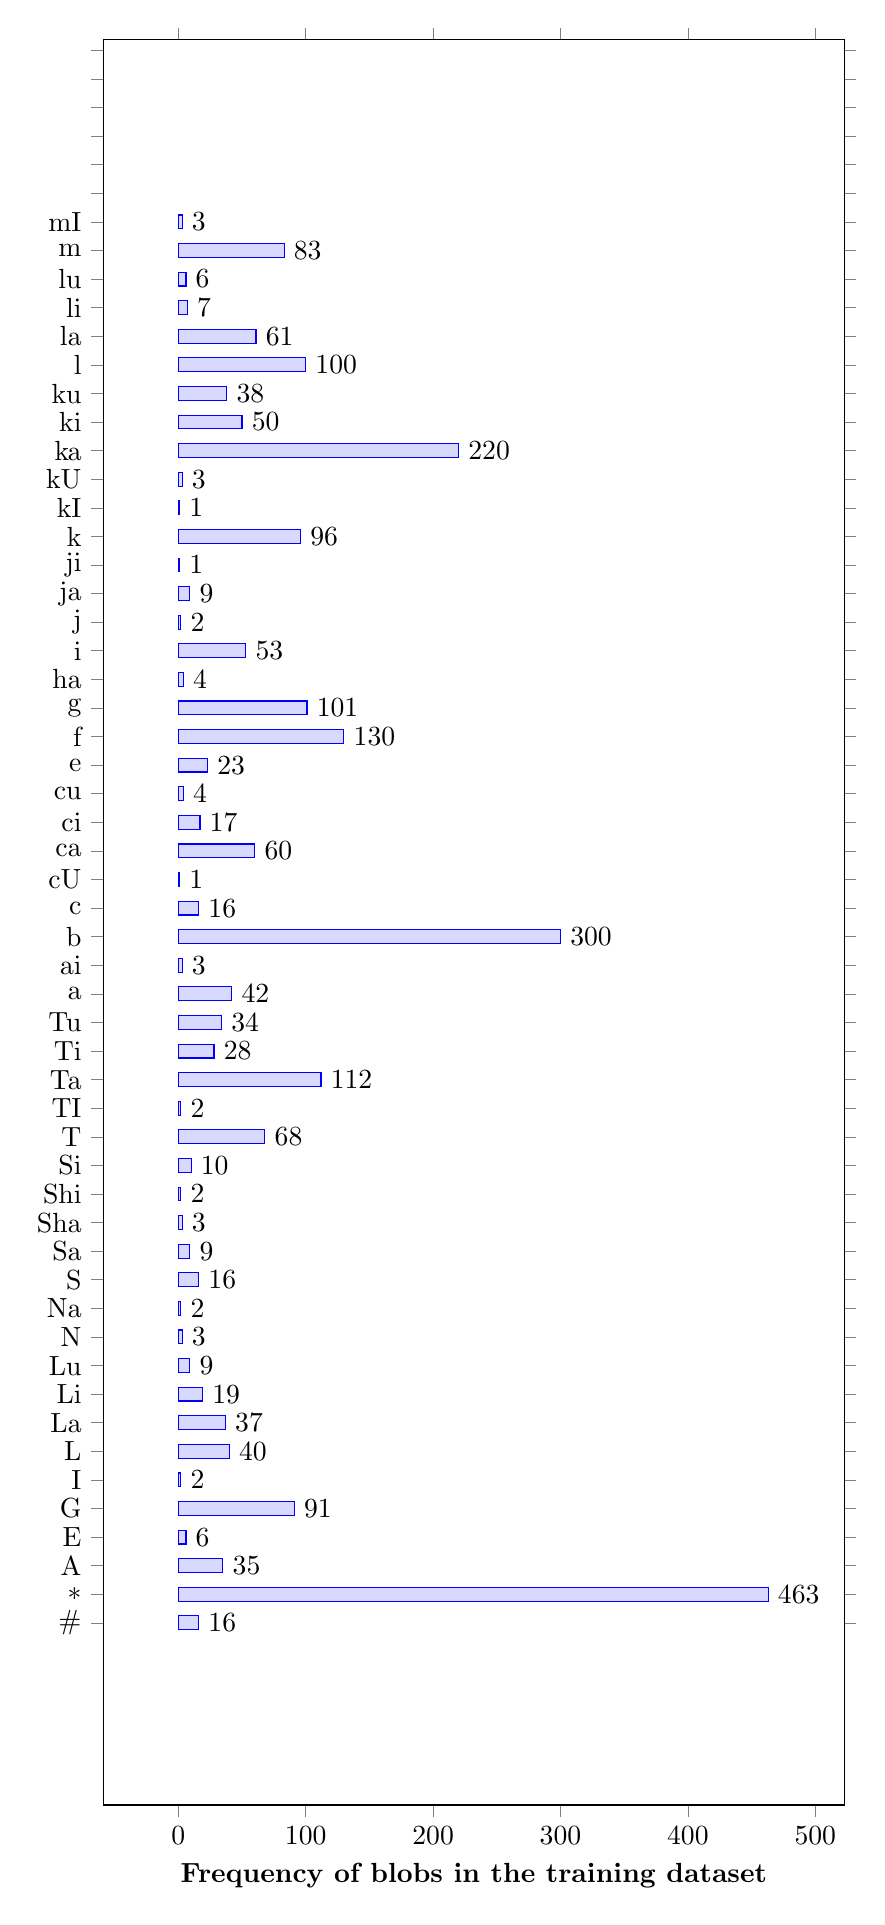
\begin{tikzpicture}[xscale=1, yscale=1]
\begin{axis}
[xbar,width=11cm,height=24cm,bar width=5pt,enlargelimits=0.13,
nodes near coords,nodes near coords
align=horizontal,
point meta=x * 1, % The displayed number.
legend pos=south east,
xlabel=\textbf{Frequency of blobs in the training dataset},
tick align=outside,
xtick={0,100,...,600}, ytick={1,...,155},
 yticklabels={\#,$*$,A,E,G,I,L,La,Li,Lu,N,Na,S,Sa,Sha,Shi,Si,T,TI,Ta,Ti,Tu,a,ai,b,c,cU,ca,ci,cu,e,f,g,ha,i,j,ja,ji,k,kI,kU,ka,ki,ku,l,la,li,lu,m,mI}
]
\addplot[draw=blue, fill=blue!15] coordinates 
{ (16,1) (463,2) (35,3) (6,4) (91,5) (2,6) (40,7) (37,8) (19,9) (9,10) (3,11) (2,12) (16,13) (9,14) (3,15) (2,16) (10,17) (68,18) (2,19) (112,20) (28,21) (34,22) (42,23) (3,24) (300,25) (16,26) (1,27) (60,28) (17,29) (4,30) (23,31) (130,32) (101,33) (4,34) (53,35) (2,36) (9,37) (1,38) (96,39) (1,40) (3,41) (220,42) (50,43) (38,44) (100,45) (61,46) (7,47) (6,48) (83,49) (3,50)  };
\end{axis}
\end{tikzpicture}


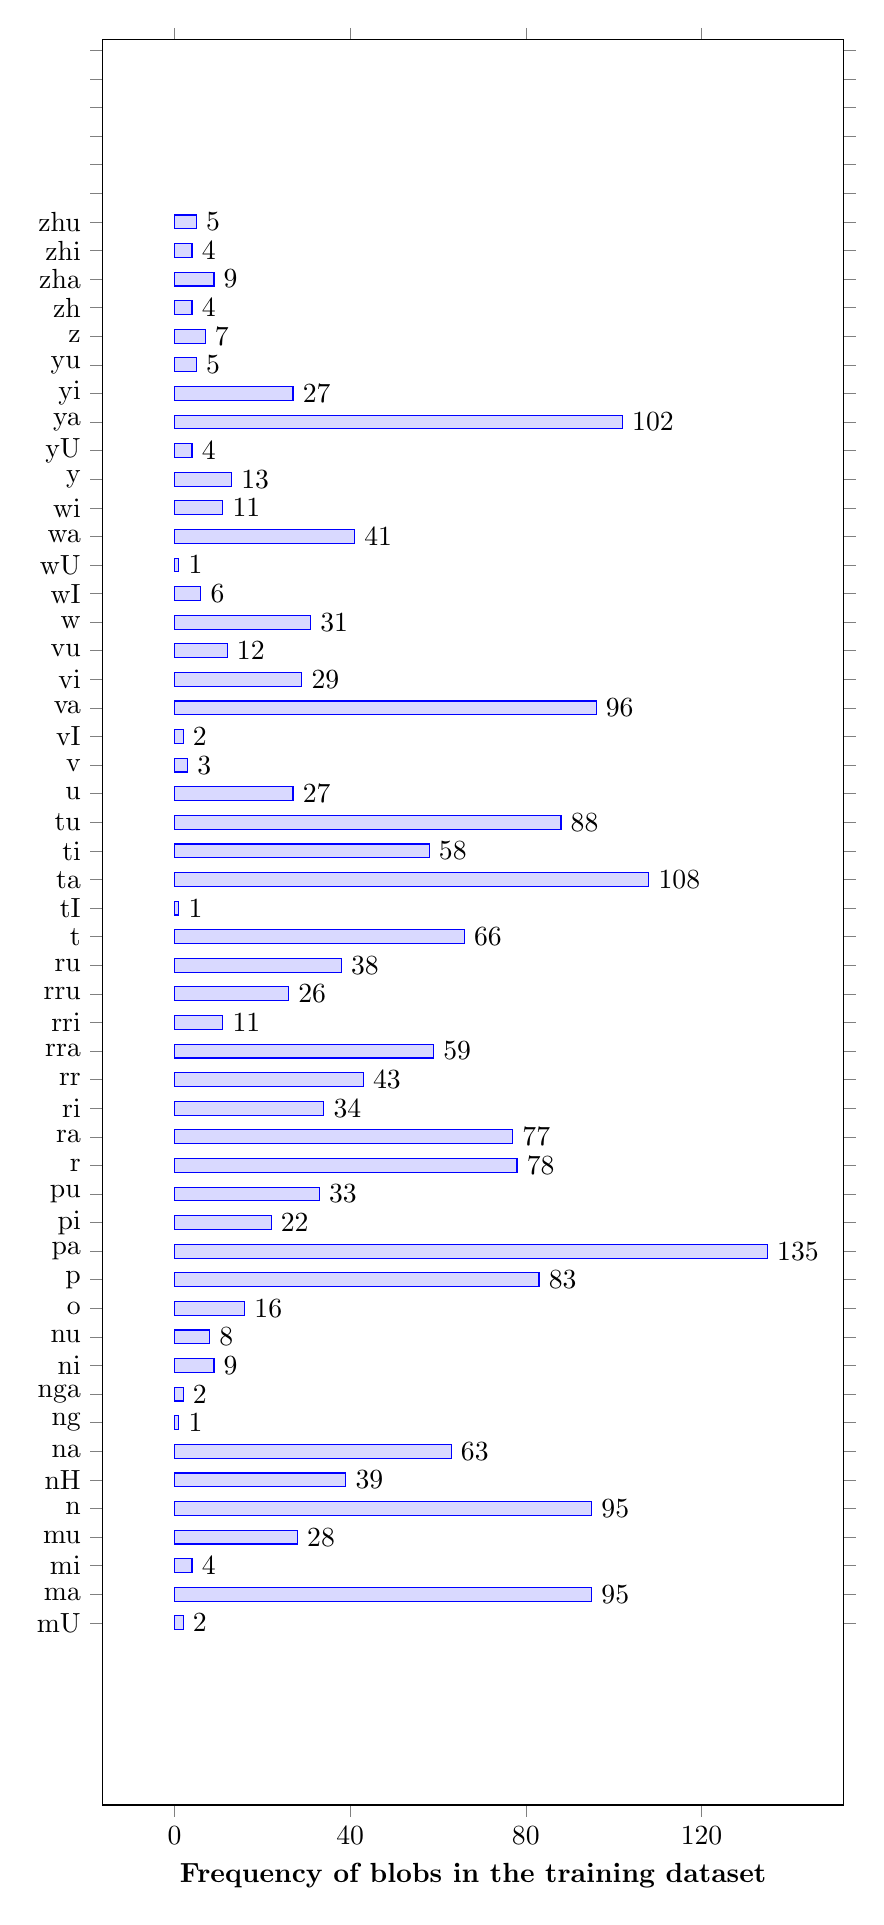
\begin{tikzpicture}[xscale=1, yscale=1]
\begin{axis}
[xbar,width=11cm,height=24cm,bar width=5pt,enlargelimits=0.13,
nodes near coords,nodes near coords
align=horizontal,
point meta=x * 1, % The displayed number.
legend pos=south east,
xlabel=\textbf{Frequency of blobs in the training dataset},
tick align=outside,
xtick={0,40,...,160}, ytick={1,...,155},
 yticklabels={mU,ma,mi,mu,n,nH,na,ng,nga,ni,nu,o,p,pa,pi,pu,r,ra,ri,rr,rra,rri,rru,ru,t,tI,ta,ti,tu,u,v,vI,va,vi,vu,w,wI,wU,wa,wi,y,yU,ya,yi,yu,z,zh,zha,zhi,zhu}
]
\addplot[draw=blue, fill=blue!15] coordinates 
{(2,1) (95,2) (4,3) (28,4) (95,5) (39,6) (63,7) (1,8) (2,9) (9,10) (8,11) (16,12) (83,13) (135,14) (22,15) (33,16) (78,17) (77,18) (34,19) (43,20) (59,21) (11,22) (26,23) (38,24) (66,25) (1,26) (108,27) (58,28) (88,29) (27,30) (3,31) (2,32) (96,33) (29,34) (12,35) (31,36) (6,37) (1,38) (41,39) (11,40) (13,41) (4,42) (102,43) (27,44) (5,45) (7,46) (4,47) (9,48) (4,49) (5,50) };
\end{axis}
\end{tikzpicture}
%\begin{axis}[ legend style={draw=none}] %pgfplot

% \begin{tikzpicture}
% \begin{axis}
% [xbar stacked, stack plots=x, tick align=outside,
% width=8cm, height=16cm, bar width=10pt,
% legend style={cells={anchor=west}}, area legend,
% xlabel=\textbf{Medals Won}, ytick={1,...,5},
% yticklabels={Russia,Netherlands,France,
% South Korea,Japan}]
% \addplot[draw=black,yellow!50!brown]
% coordinates {(1,1) (1,2) (2,3) (2,4) (3,5)};
% \addlegendentry{Gold}
% \addplot[draw=black,white!60!gray]
% coordinates {(1,1) (2,2) (0,3) (0,4) (1,5)};
% \addlegendentry{Silver}
% \addplot[draw=black,orange!70!gray]
% coordinates {(1,1) (0,2) (1,3) (3,4) (3,5)};
% \addlegendentry{Bronze}
% \end{axis}
% \end{tikzpicture}
\subsection{Custom tools}
As part of the project, a blob extractor was developed. It can extract the blob based on the bounding
box information given by tesseract. The ground truth was generated with the help of
an handy interface developed in PyGTK.
  \begin{figure}\centering
\includegraphics[scale=0.3]{./img/blobs} 
  \caption{Sample output after preprocessing}\label{BLOBIMG}
\end{figure}


\begin{figure}\centering
\includegraphics[scale=0.5]{./img/train} 
  \caption{Ground truth generation}\label{GRTR}
\end{figure}

\begin{figure}\centering
\includegraphics[scale=0.3]{./img/model} 
  \caption{Model presented to the recognition engine}\label{MODEL}
  \end{figure}

\begin{figure}\centering
\includegraphics[scale=0.7]{./img/model_gen} 
  \caption{Model generation uses one instance of each of these class}\label{MGEN}
  \end{figure}

\subsection{Elusive samples}
We inspected sample blobs for hierarchal classification. Here are some of the elusive cases
It is called so because noise or improper segmentation makes them stray blobs. Normal contour 
for class 'ya' is one. But in the figure \ref{ESAM} it is three. 
\begin{center}
\begin{figure}\centering

% \begin{tabular}{ | c | c |}
\begin{tabular}{ cc }
% \hline
\includegraphics[scale=0.4]{./img/ya} &
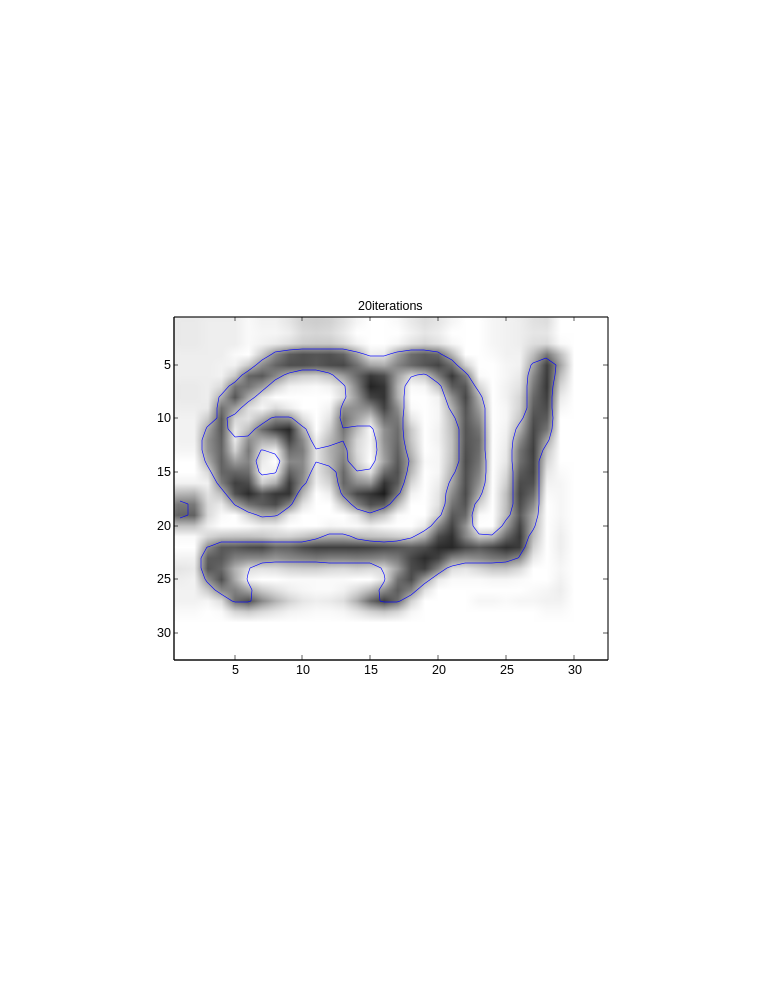
\includegraphics[scale=0.4]{./img/nu} \\ 
% \hline
\includegraphics[scale=0.4]{./img/tu} &
\includegraphics[scale=0.4]{./img/la} \\
% \hline
\end{tabular}


  \caption{Some sample elusive contour from dataset}\label{ESAM}
\end{figure}
\end{center}
\subsection{Confusion matrix}
The confusion matrix is generated with the help of ground truth and some handy shell scripts.
\begin{figure}\centering
\includegraphics[scale=0.7]{./img/confuse}
  \caption{Sample confusion matrix}\label{CONF}
\end{figure}
\subsection{Statistics}
The results are based on training and testing dataset generated as part of this project. It is a
comparison of supervised and unsupervised technique for character recognition. It should be noted that
tesseract doesn't perform perfect segmentation as expected because of touching characters. 
So junk and improper segmentation of blobs are removed from training and testing dataset. 
However, there are some stray characters in the dataset due to the reason stated above. So the 
accuracy is calculated excluding the stray characters.
\begin{table}[!t]\center
% \scriptsize

\begin{tabular}{ | l | l | l | l | l | l | l |}
\hline
& & &  \multicolumn{2}{|c|}{Samples}&\multicolumn{2}{|c|}{Accuracy} \\ \hline
S.No & Method & Features &  Training &Testing & Training & Testing \\ \hline
1* & SVMTC & 555 & 4201 & 4067 & 75 & $<$ 44 (3 classes) \\ \hline
2** & RPT & 1000 & 155 classes& 4201 & 98 & 59 \\
\hline
\end{tabular}
\caption{Recognition result based on SVMTC and RPT } \label{RES}
\end{table}
%         \begin{itemize}
% 	  \item Legend
%   \item *Structural and Statistical features (SVM trainer and classifier is used for classification)
% \item **Random Projection (L2-norm is used for recognition)
%       \end{itemize}
